% 2.3
\subsection{無順序木パターン}
\textbf{無順序木(unordered tree)}とは,後述する順序木と異なり同じ親を持つ頂点に順序関係(兄弟関係)を持たない木のことである.図\ref{fig:sibling_relationship}の2つの木は描き方は異なるが同じ木と扱われる.

% 定義1
\begin{define}{\bf 無順序木における変数}\par
  $\ell$を1以上の整数とする.$T=(V_T,E_T)$の変数とは,次の条件(1)--(3)を満たす$V_T$に含まれる頂点のリスト$h=[v_0,v_1,\ldots,v_{\ell}]$である.
  \begin{enumerate}
    \item[(1)] 頂点$v_0$は子を持つ.
    \item[(2)] $v_1,v_2,\ldots,v_{\ell}$ $(v_i \in V_T, 1\leq i\leq \ell)$は$v_0$の子である.% 順序木のときは「の連続した子である」
    \item[(3)] 変数$h$にはランクが$\ell+1$の変数ラベル$x\in X$がラベル付けされている.
  \end{enumerate}
  $v_0$を変数$h$の親ポート,$v_1,v_2,\ldots,v_{\ell}$を変数$h$の子ポートと呼ぶ.変数の次元とは,その変数に含まれる頂点数のことである.従って,変数$h=[v_0,v_1,\ldots,v_{\ell}]$の次元は$\ell+1$である.\par
  本論文では,変数を図\ref{fig:variable}のように四角で表す.四角に囲まれた文字は変数ラベルを表し,その変数が含む頂点を四角と数字付きの線で結ぶ.数字は変数におけるその頂点の順番を表す.線上の数字は,子ポートの数が1のときは省略する.
  図\ref{fig:variable}では変数ラベル$x$を持つ変数$h=[v_0,v_1,v_2,v_3]$を表す.$h$の次元は4である.
\end{define}

% 図2.2
\begin{figure}[tb]
  \centering
  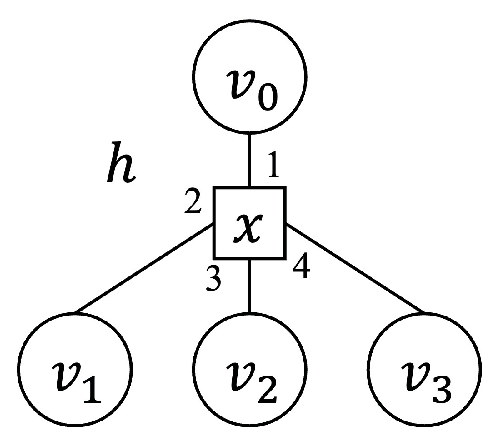
\includegraphics[scale=0.28]{fig/fig-variable.eps}
  \caption{変数ラベル$x$を持つ変数$h=[v_0,v_1,v_2,v_3]$}\label{fig:variable}
\end{figure}

% 定義2
\begin{define}{\bf 無順序項木パターン(unordered term tree pattern)}\par
  $T=(V_T,E_T)$を無順序木とし,$H_T$を$T$の変数の集合とする.ただし,任意の異なる2つの変数$h_1,\,h_2\in H_T$に対して,$h_1$と$h_2$に共通して現れる頂点は高々1つであるとする.無順序項木パターンとは,次の条件(1)--(4)を満たす3つ組$t=(V_t,E_t,H_t)$である:
  \begin{enumerate}
    \item[(1)] $V_t=V_T$,
    \item[(2)] $E_t=E_T\setminus \left(\bigcup_{[v_0,v_1,\ldots,v_{\ell}]\in H_T}\{(v_0,v_i)\in E_T\mid 1\leq i\leq \ell\}\right)$,
    \item[(3)] $H_t=H_T$,
    \item[(4)] $V_t$に属す頂点の頂点ラベル,$E_t$に属す辺の辺ラベルは,それぞれに対応する$V_T$の頂点ラベル,$E_T$の辺ラベルと同じである.
  \end{enumerate}
\end{define}

% 定義2
\begin{define}{\bf 無順序項木パターンの束縛と代入}\par
  $x\in X$をランク$\ell+1$の変数ラベル,$g$を$\ell+1$個以上の頂点を持つ無順序項木パターンとする.$u_0$を$g$の根とし,$u_1,\ldots,u_{\ell}$を$g$の根以外の互いに異なる$\ell$個の頂点とし,$\sigma=[u_0,u_1,\ldots,u_{\ell}]$とする.このとき,形式$x:=[g,\sigma]$を$g$の$\sigma$による$x$への\textbf{束縛(binding)}または単に$x$の束縛という.
  $f=(V_{f},E_{f},H_{f})$を無順序項木パターンとする.ランク$\ell+1$の変数ラベル$x$を持つ変数が$f$に存在するとき,その変数を$h_1,\ldots,h_k$ $(k\geq 0)$とする.束縛$x:=[g,\sigma]$を変数$h_1,\ldots,h_k$に次のように同時に適用して得られる無順序項木パターンを$f\{x:=[g,\sigma]\}$と書く:
  \begin{enumerate}
    \item[(1)] $g_1,\ldots,g_k$を無順序項木パターン$g$と同型な無順序項木パターンとする.
    \item[(2)] 変数$h_j=[v_0^{(j)},v_1^{(j)},\ldots,v_{\ell}^{(j)}]$ $(1\leq j\leq k)$に関して,$H_f$から変数$h_j$を削除し,$g$の頂点$u_0,u_1,\ldots,u_{\ell}$に対応する$g_j$の頂点$u_0^{(j)},u_1^{(j)},\ldots,u_{\ell}^{(j)}$を,この順序で変数$h_j$の頂点$v_0^{(j)},v_1^{(j)},\ldots,v_{\ell}^{(j)}$と同一視する.同一視後の頂点ラベルは,頂点$v_0^{(j)},v_1^{(j)},\ldots,v_{\ell}^{(j)}$の頂点ラベルを継承する.
  \end{enumerate}
  \textbf{代入(substitution)}とは,$x_i\,(1\leq i\leq n)$が$X$の異なる変数ラベルであるような束縛の有限集合$\theta=\{x_1:=[g_1,\sigma_1],\ldots,x_n:=[g_n,\sigma_n]\}$である.
  ただし,$g_{1},\ldots,g_{n}$には変数ラベル$x_1,\ldots,x_n$を持つ変数が現れないと仮定する.
  代入$\theta$による$f$の\textbf{インスタンス(instance)}とは,$f$に対して,$\theta$の全ての束縛$x_i:=[g_i,\sigma_i]$ $(1\leq i\leq n)$を適用して得られる無順序項木パターンである.代入$\theta$による$f$のインスタンスを$f\theta$と書く.

  無順序木(順序木) $T_1$と$T_2$が無順序木(順序木)として同型であるとき,$T_1\equiv T_2$と書く.

  % 図2.3
  \begin{figure}[tb]
    \centering
    \includegraphics[scale=0.28]{fig/fig-lutp.eps}
    \caption{線形無順序木パターン$t$と無順序木$t\theta \equiv T$を示す.無順序木の場合,代入後の$T$と下に示す$T_1,T_2,\ldots ,T_n$は同型である.}\label{fig:lutp} % 無順序木パターン$t$と無順序木$t\theta\equiv T$
  \end{figure}

  $\Sigma,\Lambda$をそれぞれ頂点ラベルの集合,辺ラベルの集合とする無順序木の全体を${\cal UT}_{\Sigma,\Lambda}$とする.また,$\Sigma,\Lambda,X$をそれぞれ頂点ラベルの集合,辺ラベルの集合,変数ラベルの集合とする無順序項木パターンの全体を${\cal UTTP}_{\Sigma,\Lambda,X}$とする.次のように${\cal UTTP}_{\Sigma,\Lambda,X}$の部分集合を定める:
  \begin{align*}
    {\cal LUTTP}_{\Sigma,\Lambda,X} & = \{t=(V_t,E_t,H_t)\in{\cal UTTP}_{\Sigma,\Lambda,X}\mid\\
    & \hspace*{12pt}\forall h_1,\,h_2\in H_t\,(h_1\not= h_2)\mbox{に対して,}\\
    & \hspace*{12pt}\mbox{変数}h_1\mbox{と}h_2\mbox{の変数ラベルは異なる}\},\\
    {\cal LUTP}_{\Sigma,\Lambda,X} & = \{t=(V_t,E_t,H_t)\in{\cal LUTTP}_{\Sigma,\Lambda,X}\mid\\
    & \hspace*{12pt}\forall h\in H_t\mbox{の次元は2であり,かつ}\\
    & \hspace*{12pt}\mbox{$h$の子ポートは葉である}\}.
  \end{align*}
  
  \noindent
  ${\cal LUTTP}_{\Sigma,\Lambda,X}$に属す無順序項木パターンを\textbf{線形無順序項木パターン(linear unordered term tree pattern)}と呼ぶ.また,${\cal LUTP}_{\Sigma,\Lambda,X}$に属す線形無順序項木パターンを\textbf{線形無順序木パターン(linear unordered tree pattern)}と呼ぶ.

  以降,無順序木$T=(V_T,E_T)$を,変数を持たない無順序項木パターン$T=(V_T,E_T,\emptyset)$とみなす.
\end{define}

% 定義4
\begin{define}{\bf 無順序項木パターン言語}\par
  無順序項木パターン$t\in {\cal UTTP}_{\Sigma,\Lambda,X}$に対して,$t$の無順序項木パターン言語$L(t)\subseteq {\cal UT}_{\Sigma,\Lambda}$を次のように定義する:
  $$L(t)=\{t\theta\in {\cal UT}_{\Sigma,\Lambda}\mid \mbox{$\theta$は$t$の変数への任意の代入}\}.$$
  \noindent
  線形無順序木パターン$t$に対して,$T\in L(t)$となる無順序木$T$の例を図\ref{fig:lutp}にあげる.
\end{define}


無順序項木パターン$t$と無順序木$T$に対して,代入$\theta$が存在して$t\theta\equiv T$となるとき,$t$は$T$にマッチするという.

% 定義5
\begin{define}{\bf 左深さ優先木}\par
  順序木において,左側の子を優先して深さ優先探索を行い,訪れた頂点の深さを並べた整数列を\textbf{深さ列(Depth Sequence)}と呼ぶ.順序木$T$における深さ列は$DS(T)$で表す.この深さ列は,木の構造における頂点の探索順序とその深さに基づいており,深さ優先探索における頂点訪問の順番を整数列として記録したものである.

  一方,無順序木の場合,子の順序が決まっていないため,子の順序を入れ替えることによって異なる順序木を構成することが可能である.無順序木においては,それと同型な様々な順序木表現が構成されるが,その中でも深さ列として辞書式順序で最大の値を持つものを\textbf{左深さ優先木(left depth first search tree)}と呼ぶ.この左深さ優先木がその無順序木を代表する順序木表現と考え,これを\textbf{左深さ優先無順序木(left depth first search unordered tree)}とする(図\ref{fig:left_dfs}).%左深さ優先木は,深さ優先探索において左側の子を優先的に探索するという特性を持つ.
  %具体的には,2つの無順序木が同型である場合,それらの左深さ優先木の深さ列は等しくなる.これは、無順序木の構造においてどのように子の順序を選んでも,左深さ優先木が持つ深さ列が唯一であることを意味している.
\end{define}

% 図2.4
\begin{figure*}[tb]
  \centering
  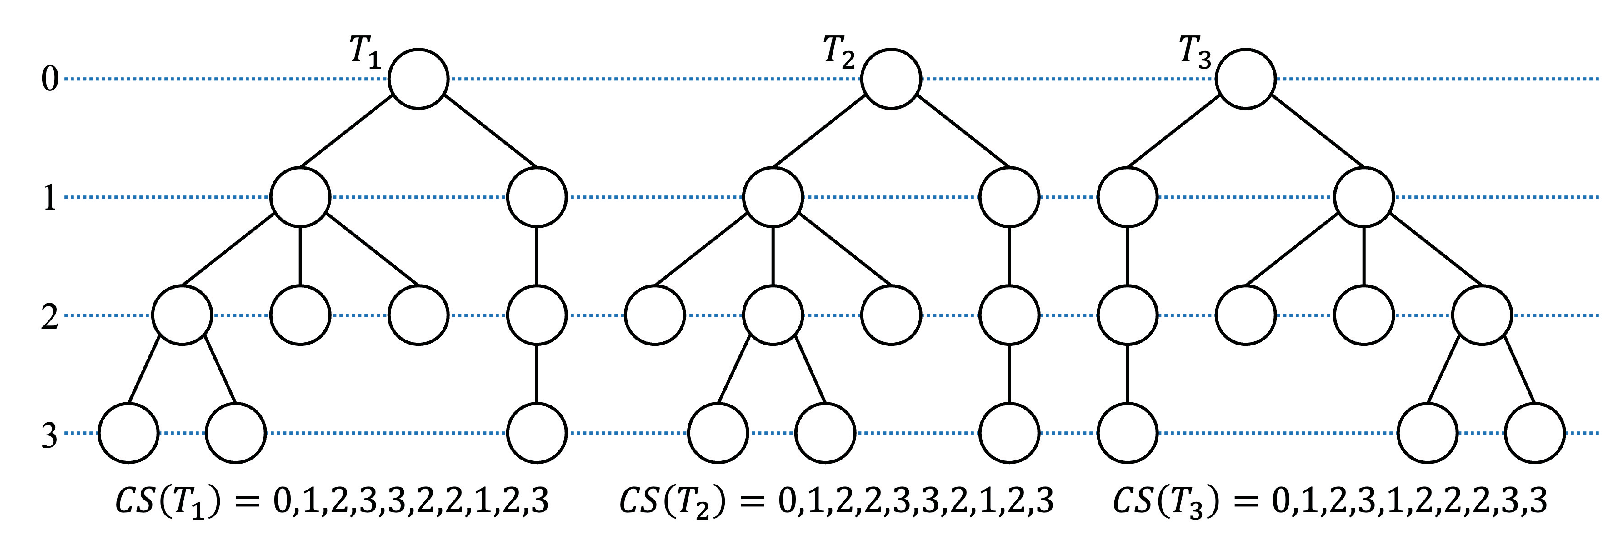
\includegraphics[scale=0.5]{fig/fig-left_dfs.eps}
  \caption{$T_1,T_2,T_3$は同型の無順序木で,左深さ優先木を定めると$T_1$に一意に定まる.}\label{fig:left_dfs}
\end{figure*}
